\documentclass[11pt,a4paper,]{article}
\usepackage{lmodern}

\usepackage{amssymb,amsmath}
\usepackage{ifxetex,ifluatex}
\usepackage{fixltx2e} % provides \textsubscript
\ifnum 0\ifxetex 1\fi\ifluatex 1\fi=0 % if pdftex
  \usepackage[T1]{fontenc}
  \usepackage[utf8]{inputenc}
\else % if luatex or xelatex
  \usepackage{unicode-math}
  \defaultfontfeatures{Ligatures=TeX,Scale=MatchLowercase}
\fi
% use upquote if available, for straight quotes in verbatim environments
\IfFileExists{upquote.sty}{\usepackage{upquote}}{}
% use microtype if available
\IfFileExists{microtype.sty}{%
\usepackage[]{microtype}
\UseMicrotypeSet[protrusion]{basicmath} % disable protrusion for tt fonts
}{}
\PassOptionsToPackage{hyphens}{url} % url is loaded by hyperref
\usepackage[unicode=true]{hyperref}
\hypersetup{
            pdftitle={Assignment 1: BEX5200 Climate Change and Carbon Management Strategies},
            pdfborder={0 0 0},
            breaklinks=true}
\urlstyle{same}  % don't use monospace font for urls
\usepackage{geometry}
\geometry{a4paper, centering, text={16cm,24cm}}
\usepackage[style=authoryear-comp,]{biblatex}
\addbibresource{references.bib}
\addbibresource{packages.bib}
\usepackage{longtable,booktabs}
% Fix footnotes in tables (requires footnote package)
\IfFileExists{footnote.sty}{\usepackage{footnote}\makesavenoteenv{long table}}{}
\IfFileExists{parskip.sty}{%
\usepackage{parskip}
}{% else
\setlength{\parindent}{0pt}
\setlength{\parskip}{6pt plus 2pt minus 1pt}
}
\setlength{\emergencystretch}{3em}  % prevent overfull lines
\providecommand{\tightlist}{%
  \setlength{\itemsep}{0pt}\setlength{\parskip}{0pt}}
\setcounter{secnumdepth}{5}

% set default figure placement to htbp
\makeatletter
\def\fps@figure{htbp}
\makeatother


\title{Assignment 1: BEX5200 Climate Change and Carbon Management Strategies}
\providecommand{\subtitle}[1]{}
\subtitle{BEX5200 Climate Change and Carbon Management Strategies}

%% MONASH STUFF

%% CAPTIONS
\RequirePackage{caption}
\DeclareCaptionStyle{italic}[justification=centering]
 {labelfont={bf},textfont={it},labelsep=colon}
\captionsetup[figure]{style=italic,format=hang,singlelinecheck=true}
\captionsetup[table]{style=italic,format=hang,singlelinecheck=true}


%% FONT
\RequirePackage{bera}
\RequirePackage[charter,expert,sfscaled]{mathdesign}
\RequirePackage{fontawesome}

%% HEADERS AND FOOTERS
\RequirePackage{fancyhdr}
\pagestyle{fancy}
\rfoot{\Large\sffamily\raisebox{-0.1cm}{\textbf{\thepage}}}
\makeatletter
\lhead{\textsf{\expandafter{\@title}}}
\makeatother
\rhead{}
\cfoot{}
\setlength{\headheight}{15pt}
\renewcommand{\headrulewidth}{0.4pt}
\renewcommand{\footrulewidth}{0.4pt}
\fancypagestyle{plain}{%
\fancyhf{} % clear all header and footer fields
\fancyfoot[C]{\sffamily\thepage} % except the center
\renewcommand{\headrulewidth}{0pt}
\renewcommand{\footrulewidth}{0pt}}

%% MATHS
\RequirePackage{bm,amsmath}
\allowdisplaybreaks

%% GRAPHICS
\RequirePackage{graphicx}
\setcounter{topnumber}{2}
\setcounter{bottomnumber}{2}
\setcounter{totalnumber}{4}
\renewcommand{\topfraction}{0.85}
\renewcommand{\bottomfraction}{0.85}
\renewcommand{\textfraction}{0.15}
\renewcommand{\floatpagefraction}{0.8}


%\RequirePackage[section]{placeins}

%% SECTION TITLES


%% SECTION TITLES (NEW: Changing sections and subsections color)
\RequirePackage[compact,sf,bf]{titlesec}
\titleformat*{\section}{\Large\sf\bfseries\color[rgb]{0.8, 0.7, 0.1 }}
\titleformat*{\subsection}{\large\sf\bfseries\color[rgb]{0.8, 0.7, 0.1 }}
\titleformat*{\subsubsection}{\sf\bfseries\color[rgb]{0.8, 0.7, 0.1 }}
\titlespacing{\section}{0pt}{2ex}{.5ex}
\titlespacing{\subsection}{0pt}{1.5ex}{0ex}
\titlespacing{\subsubsection}{0pt}{.5ex}{0ex}


%% TITLE PAGE
\def\Date{\number\day}
\def\Month{\ifcase\month\or
 January\or February\or March\or April\or May\or June\or
 July\or August\or September\or October\or November\or December\fi}
\def\Year{\number\year}

%% LINE AND PAGE BREAKING
\sloppy
\clubpenalty = 10000
\widowpenalty = 10000
\brokenpenalty = 10000
\RequirePackage{microtype}

%% PARAGRAPH BREAKS
\setlength{\parskip}{1.4ex}
\setlength{\parindent}{0em}

%% HYPERLINKS
\RequirePackage{xcolor} % Needed for links
\definecolor{darkblue}{rgb}{0,0,.6}
\RequirePackage{url}

\makeatletter
\@ifpackageloaded{hyperref}{}{\RequirePackage{hyperref}}
\makeatother
\hypersetup{
     citecolor=0 0 0,
     breaklinks=true,
     bookmarksopen=true,
     bookmarksnumbered=true,
     linkcolor=darkblue,
     urlcolor=blue,
     citecolor=darkblue,
     colorlinks=true}

\usepackage[showonlyrefs]{mathtools}
\usepackage[no-weekday]{eukdate}

%% BIBLIOGRAPHY

\makeatletter
\@ifpackageloaded{biblatex}{}{\usepackage[style=authoryear-comp, backend=biber, natbib=true]{biblatex}}
\makeatother
\ExecuteBibliographyOptions{bibencoding=utf8,minnames=1,maxnames=3, maxbibnames=99,dashed=false,terseinits=true,giveninits=true,uniquename=false,uniquelist=false,doi=false, isbn=false,url=true,sortcites=false}

\DeclareFieldFormat{url}{\texttt{\url{#1}}}
\DeclareFieldFormat[article]{pages}{#1}
\DeclareFieldFormat[inproceedings]{pages}{\lowercase{pp.}#1}
\DeclareFieldFormat[incollection]{pages}{\lowercase{pp.}#1}
\DeclareFieldFormat[article]{volume}{\mkbibbold{#1}}
\DeclareFieldFormat[article]{number}{\mkbibparens{#1}}
\DeclareFieldFormat[article]{title}{\MakeCapital{#1}}
\DeclareFieldFormat[article]{url}{}
%\DeclareFieldFormat[book]{url}{}
%\DeclareFieldFormat[inbook]{url}{}
%\DeclareFieldFormat[incollection]{url}{}
%\DeclareFieldFormat[inproceedings]{url}{}
\DeclareFieldFormat[inproceedings]{title}{#1}
\DeclareFieldFormat{shorthandwidth}{#1}
%\DeclareFieldFormat{extrayear}{}
% No dot before number of articles
\usepackage{xpatch}
\xpatchbibmacro{volume+number+eid}{\setunit*{\adddot}}{}{}{}
% Remove In: for an article.
\renewbibmacro{in:}{%
  \ifentrytype{article}{}{%
  \printtext{\bibstring{in}\intitlepunct}}}

\AtEveryBibitem{\clearfield{month}}
\AtEveryCitekey{\clearfield{month}}

\makeatletter
\DeclareDelimFormat[cbx@textcite]{nameyeardelim}{\addspace}
\makeatother

\author{\sf\Large\textbf{ Mohammed Faizan}\\ {\sf\large MBAt\\[0.5cm]}}

\date{\sf\Date~\Month~\Year}
\makeatletter
\lfoot{\sf Faizan: \@date}
\makeatother


%%%% PAGE STYLE FOR FRONT PAGE OF REPORTS

\makeatletter
\def\organization#1{\gdef\@organization{#1}}
\def\telephone#1{\gdef\@telephone{#1}}
\def\email#1{\gdef\@email{#1}}
\makeatother
  \organization{Monash University}

  \def\name{Climate Works Australia\newline Mohammed Faizan}

  \telephone{(03) 9905 2478}

  \email{questions@company.com}                 %NEW: New email addresss

\def\webaddress{\url{http://company.com/stats/consulting/}} %NEW: URl
\def\abn{12 377 614 630}                                    % NEW: ABN
\def\logo{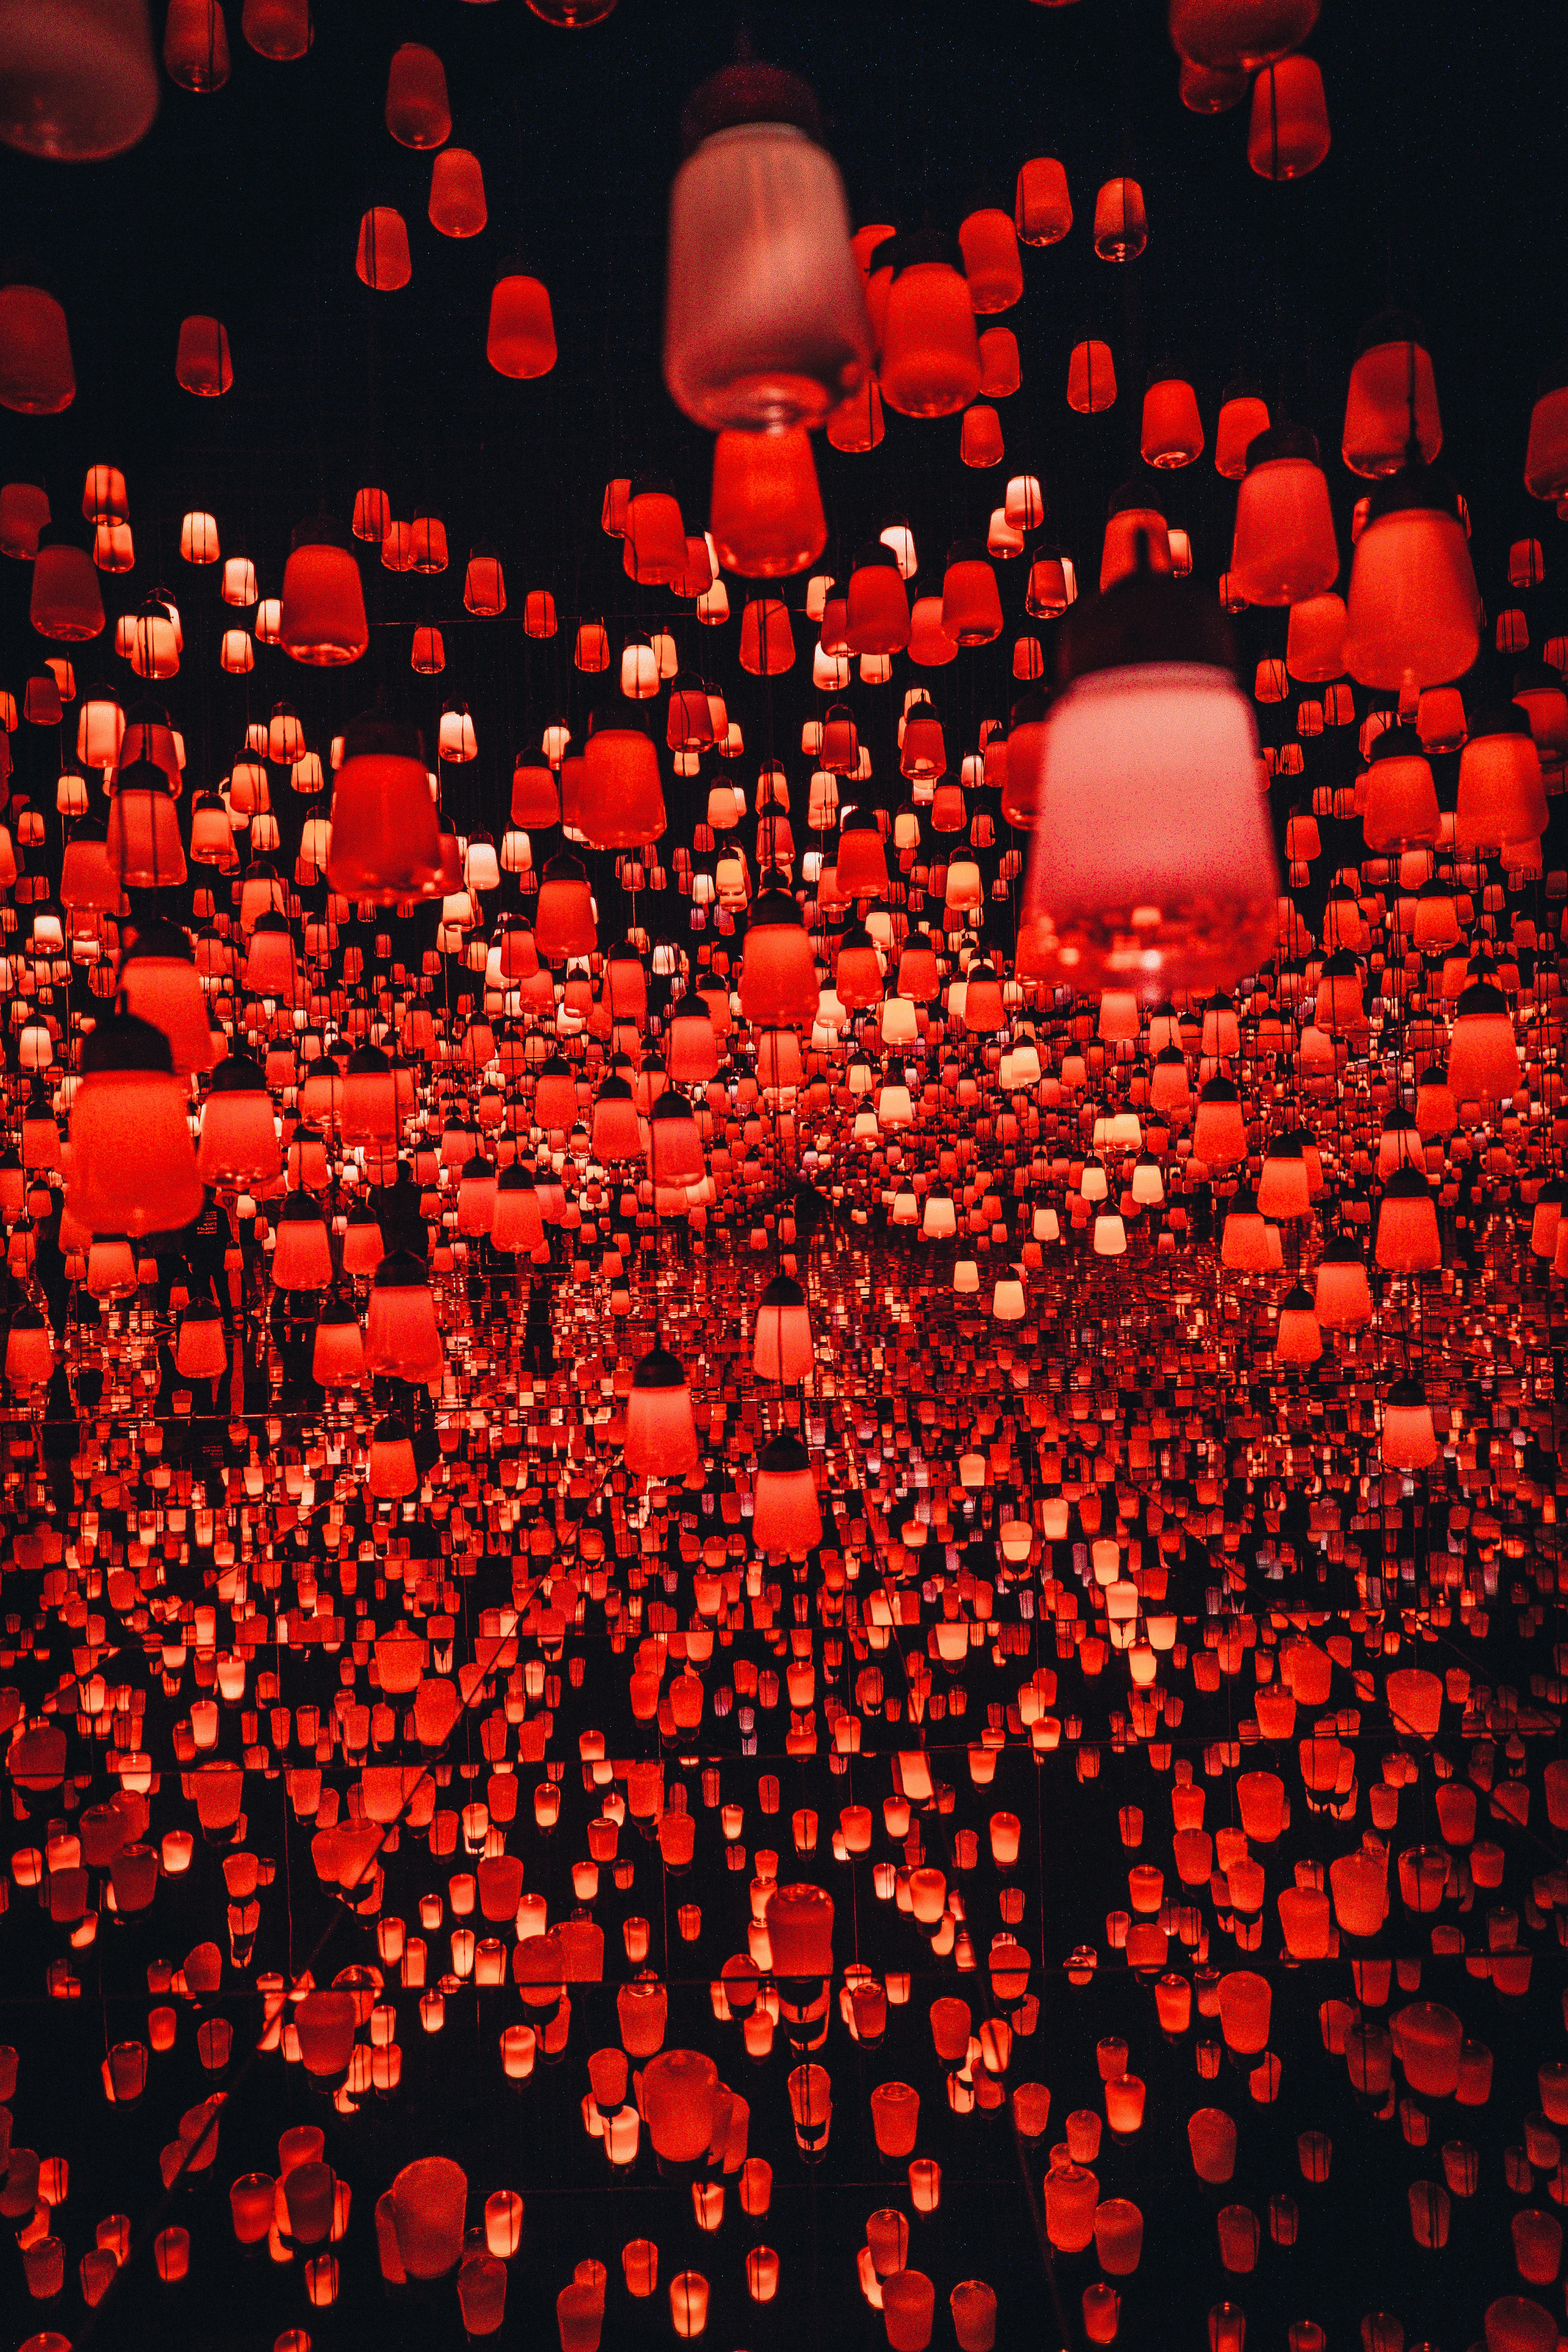
\includegraphics[width=6cm]{Figures/logo}}  %NEW: Changing logo
\def\extraspace{\vspace*{1.6cm}}
\makeatletter
\def\contactdetails{\faicon{phone} & \@telephone \\
                    \faicon{envelope} & \@email}
\makeatother

%%%% FRONT PAGE OF REPORTS

\def\reporttype{Report for}

\long\def\front#1#2#3{
\newpage
\begin{singlespacing}
\thispagestyle{empty}
\vspace*{-1.4cm}
\hspace*{-1.4cm}
\hbox to 16cm{
  \hbox to 6.5cm{\vbox to 14cm{\vbox to 25cm{
    \logo
    \vfill
    \parbox{6.3cm}{\raggedright
      \sf\color[rgb]{0.8, 0.7, 0.1 }    % NEW color 
      {\large\textbf{\name}}\par
      \vspace{.7cm}
      \tabcolsep=0.12cm\sf\small
      \begin{tabular}{@{}ll@{}}\contactdetails
      \end{tabular}
      \vspace*{0.3cm}\par
      ABN: \abn\par
    }
  }\vss}\hss}
  \hspace*{0.2cm}
  \hbox to 1cm{\vbox to 14cm{\rule{4pt}{26.8cm}\vss}\hss\hfill}  %NEW: Thicker line
  \hbox to 10cm{\vbox to 14cm{\vbox to 25cm{   
      \vspace*{3cm}\sf\raggedright
      \parbox{11cm}{\sf\raggedright\baselineskip=1.2cm
         \fontsize{24.88}{30}\color[rgb]{0, 0.29, 0.55}\sf\textbf{#1}}   % NEW: title color blue
      \par
      \vfill
      \large
      \vbox{\parskip=0.8cm #2}\par
      \vspace*{2cm}\par
      \reporttype\\[0.3cm]
      \hbox{#3}%\\[2cm]\
      \vspace*{1cm}
      {\large\sf\textbf{\Date~\Month~\Year}}
   }\vss}
  }}
\end{singlespacing}
\newpage
}

\makeatletter
\def\titlepage{\front{\expandafter{\@title}}{\@author}{\@organization}}
\makeatother

\usepackage{setspace}
\setstretch{1.5}

%% Any special functions or other packages can be loaded here.
\AtBeginDocument{\addtocontents{toc}{\protect\thispagestyle{empty}}} 
\usepackage{capt-of}
\usepackage{graphicx}
\usepackage{url}
\usepackage{float}
\usepackage{booktabs}
\usepackage{longtable}
\usepackage{array}
\usepackage{multirow}
\usepackage{wrapfig}
\usepackage{float}
\usepackage{colortbl}
\usepackage{pdflscape}
\usepackage{tabu}
\usepackage{threeparttable}
\usepackage{threeparttablex}
\usepackage[normalem]{ulem}
\usepackage{makecell}
\usepackage{xcolor}


\begin{document}
\titlepage

{
\setcounter{tocdepth}{2}
\tableofcontents
}
\newpage

\hypertarget{report-evaluation-of-business-ambition-for-1.5-through-science-based-targets-initiative-commitment-made-by-worley-australia}{%
\section{Report: Evaluation of Business Ambition for 1.5 through SCIENCE BASED TARGETS INITIATIVE commitment made by Worley, Australia}\label{report-evaluation-of-business-ambition-for-1.5-through-science-based-targets-initiative-commitment-made-by-worley-australia}}

The forces of change, climate change, energy transition, circular economy, and digitalization of industries have compelled establishments to reform and develop sustainable operations. Energy, oil and gas industries are the sectors where this change is felt more rapidly. ``Worley, is a leading global provider of professional services headquartered in Australia, delivering project and asset services in the energy, chemicals and resources sectors around the world'' (\textcite{sustainabilityreport2020}). Figure \ref{fig:totalcarbonemissions} shows the Energy Usage and GHG Emissions of Worley. There was a drop prior to 2019, however energy consumption and GHG emissions have risen significantly in 2020. Worley states the acquisition of Jacobs Engineering Group Inc which doubled their business operation as the reason for this surge. This report explores the climate action and sustainable developments made by Worley and the significance of these commitments in the context of climate change, business motives and the risks and opportunities associated with it.

\begin{figure}[H]
\includegraphics[width=7in, height = 2in]{Figures/emissionhistory}
\includegraphics[width=7in, height = 2in]{Figures/energyusageandemissions.png}
\caption{Energy Usage and GHG Emissions}
\label{fig:totalcarbonemissions}
\end{figure}

Worley prides itself with a worldwide network of over 48,000 consultants, engineers, construction workers and data scientists coming together to solve the complexity of the energy, chemicals and resources sectors including turnkey projects that cover the full life-cycle from creating, sustaining and enhancing assets right through to decommissioning and rehabilitation for a sustained economic, social and environmental progress for communities across the world. \textbf{Worley is committed to \textcite{businessambition} through \textcite{aboutsbti}}(\textcite{sciencebasedtargets}) to reach net zero by reducing emissions and waste in its projects and operations. The company has committed to report its performance annually through its sustainability report.

\begin{figure}

{\centering \includegraphics[width=0.75\linewidth]{/Users/mohammedfaizan/git/bex5200/assignment1/BEX5200_Assignment1/Figures/roadmap} 

}

\caption{Road Map towards Net Zero by 2030}\label{fig:roadmap}
\end{figure}

Worley is dependent heavily on its clients as it delivers turnkey projects across all sectors of energy and chemicals. Climate commitments become significant as there is dependency involved. Worley must be part of brown field projects based on the needs of the client and the project. It is therefore only apt for Worley to commit to \textcite{businessambition} through \textcite{aboutsbti}, to scientifically evolve sustainable operations through emission reduction and energy transition. Worley aids its customers who are under pressure to deliver, develop, digitize and decarbonize. The aims of the commitment are in alignment with the Paris Agreement, to achieve net zero by 2050 for its scope 3 emissions. In addition, it promotes Circular Economy, to re-purpose goods or recycle them into something else.

\begin{figure}

{\centering \includegraphics[width=0.75\linewidth]{/Users/mohammedfaizan/git/bex5200/assignment1/BEX5200_Assignment1/Figures/helpingcustomers} 

}

\caption{Worley is committed to achieving net zero Scope 1 and Scope 2 greenhouse gas emissions by 2030, and to pro-actively supporting our customers to reduce emissions on their projects and assets. We will keep our stakeholders informed of our strategy and progress against established metrics, including the recommendations of the Task Force on Climate-related Financial Disclosure.- [Worley](https://www.worley.com/sustainability/environment/climate-change)}\label{fig:helpingcustomers}
\end{figure}

Climate change affects business and life in unanticipated ways from rising temperatures, uneven rainfall pattern to extreme weather. With the growing population, a 10\% increase in energy demand is projected by 2030. These impacts have led government, organisations and businesses to embed climate policies and comply with the Paris agreement. Worley's customers range from oil and gas, power, Refining and Chemicals to Mining, Minerals \& Metals and hence the motive for energy transition, circular economy and other science based target initiatives present a business opportunity for Worley at the same time fulfilling its commitments. Worley has accepted change and thus is more inclined towards sustainable growth of the environment and the communities in which they operate.

Worley has incorporated climate change action and commits towards energy transition and to support its customers for a low-carbon future as its key business strategy. Risk and opportunities are identified in the market for the company to capitalise on the opportunties in energy transition and to mitigate risks associated associated with transitioning industries. ``Worley uses the \href{https://www.iea.org/}{International Energy Agency} Sustainable Development Scenario \textcite{iea} for strategic planning and develops business resiliency pathways accordingly across its portfolio of businesses and geographies'' \textcite{sustainabilityreport2020}. And their R3 group support businesses in response to physical risks such as extreme weather and rising temperature.

Worley is already investing in renewable energy technology, which is transforming the power sector at an unprecedented rate and designing future-ready infrastructure that can adapt to uses like green hydrogen production(Burning hydrogen gives water vapour and it can be used to store excess energy). This inherently causes increased attention to deliver future economic returns and to optimise performance and operational cost of existing assets to ensure their competency ahead. The significant cost reduction by use of renewable energy(solar and wind), and distributed power generation systems have motivated the shift from fossil fuels.

Worley is ``working on gray, blue and green hydrogen projects all over the world, from studies on the feasibility of crude oil to hydrogen pathways in the Middle East to a detailed study of green hydrogen to ammonia in Australia, and the engineering, procurement and construction of a green hydrogen refueling station in New Zealand.'' \textcite{sustainabilityreport2020}

Cost reduction in Hydrogen Production (Business Motive): The collaboration with Queensland Nitrates (QNP) and Neoen in Queesnsland to complete a feasibility study to determine commercial production of green hydrogen for its largest use domestic and internationally, ammonia production. Worley has setup a digital business model, VECKTA,to optimize Distributed Energy System(DES) with \href{https://xendee.com/}{XENDEE}. VECKTA is a virtual marketplace for people and companies for the design, technology and sales of DES. Natural gas will play a key role until the mid 2020s in fuel switching and is a bridge to decarbinised energy supply. And, Worley aims to develop projects to ``enable communities to develop economically via productive use of natural resources, skills development and lifting communities out of energy poverty''(\textcite{sustainabilityreport2020}) in the energy, chemicals and resources sectors internationally.

The key performance indicators for Worley's climate commitments include ``Net zero road map, Worley Foundation, People network groups, Sustainable Solutions process'' \textcite{sustainabilityreport2020} and the TCFD framework for recommendation of the risk, opportunities and progress. The digital platform, Requis speeds up procurement process and thereby eliminates waste by using and re-using equipment. As companies race towards net zero, the infrastructure(obselete) plays a vital role in production rate and commodity prices. The Maintenance, Modifications and Operations (MMO) unit of Worley helps its customers to deliver increased productivity in cleaner ways, thereby achieving potential project costs.

\begin{figure}[H]
\includegraphics[width=5in, height = 2.5in]{Figures/reporting}
\includegraphics[width=5in, height = 2.5in]{Figures/shift}
\caption{Reporting the Shift}
\label{fig:reporting}
\end{figure}

To start-off Worley conducted a survey in FY2020 to assess its sustainable growth objectives for its shareholders, customers, internal members and community partners and noted UN's ``SDG 7: Affordable and clean energy and SDG 13: Climate Action'' \textcite{sdg} was most favored. Worley claims to support economic growth by creating employment and supporting its customers in their projects. These objectives are being implemented by continued support to customers to navigate the energy transition, strategic acquisition and joint venture in solar, on-shore and off-shore wind and distributed energy systems and other projects like providing clean energy to people living in poverty in India with aid from the Pollinate Group.

The Climate Change Position Statement(CCP) reports the climate commitments and the progress being made and the Sustainable Solutions process overlooks this progress, ``featuring a carbon calculator, to measure carbon savings; and the Value Creation platform, which captures ideas and reports on those savings, it empowers Worley to identify opportunities to reduce the carbon impact of its customers' projects and to measure savings.'' \textcite{sustainabilityreport2020}. The Worley Waste Warriors was started in December 2019 to reduce the waste and carbon footprint produced in its offices and improve energy and water efficiency. The Worley Foundation donated more than \$130,000 to the Red Cross Australian bushfire disaster relief and recovery campaign. "\href{https://www.worley.com/our-work/australian-antarctic-climate-change-research}{The Worley Foundation supports scientific research in the Antarctic, Sub Antarctic and Southern Ocean as a Trailblazer10 Corporate Supporter of the Antarctic Science Foundation (ASF)" to support krill research for the Australian government's Antarctic Division."}. The Worley Foundation, through its web based tool,has partnered with Transparency International's (TI) Accountable Mining Program to help address corruption risks in the mining approvals process.

\begin{figure}[H]
\includegraphics[width=4in, height = 1in]{Figures/donations}
\caption{Donations}
\label{fig:donations}
\end{figure}

There are \href{https://sciencebasedtargets.org/companies-taking-action?sector=Construction\%20and\%20Engineering\&ambitionToggle=1\#table}{25 companies} who have committed to the Business Ambition for 1.5°C in the Construction and Engineering sector on the SBTi organisation. However, Worley stands out in this regard as it is projected towards reducing its own emissions and further aiding its customers towards net zero future. The projects and investments in green technology, energy transition and reducing direct carbon emissions through carbon capture, utilization and storage (CCUS) are a standing proof of its seriousness in this regard. The \href{https://www.enr.com/toplists/2020-Top-200-Environmental-Firms-Preview}{Engineering News Record} reports EPC companies rank based on percentage of gross revenue reported from environmental services in the preceding year. \href{https://www.enr.com/toplists/2019-Top-200-Environmental-Firms-1}{WORLEYPARSONS LTD(former name) retained its position at 59} in 2018 and 2019. The top 10 companies for environment related revnue is listed in table \ref{tab:enr} \textcite{enr}.

\begin{table}[!h]

\caption{\label{tab:enr}ENR Top 10 Environmental Firms}
\centering
\begin{tabular}[t]{l|l|l|l}
\hline
RANK 2019 & RANK 2018 & FIRM & TYPE OF WORK\\
\hline
1 & 1 & AECOM, New York, N.Y. & DES-CSL-CM/PM\\
\hline
2 & 2 & JACOBS, Dallas, Texas & CSL\\
\hline
3 & 3 & CLEAN HARBORS INC., Norwell, Mass. & OTH1\\
\hline
4 & 4 & TETRA TECH INC., Pasadena, Calif. & CSL\\
\hline
5 & 5 & FLUOR CORP., Irving, Texas & CON\\
\hline
6 & 6 & BECHTEL CORP., Reston, Va. & CON\\
\hline
7 & 8 & SALINI IMPREGILO SPA, Milan, Italy & CON\\
\hline
8 & 7 & STANTEC INC., Edmonton, Alberta, Canada & DES\\
\hline
9 & 10 & SUEZ NORTH AMERICA, Paramus, N.J. & OPS\\
\hline
10 & 9 & WOOD PLC, Houston, Texas & CON\\
\hline
\end{tabular}
\end{table}

\newpage

And, the ranking in Australia is displayed below, and Worley ranks second in Australia.

\begin{table}[!h]

\caption{\label{tab:aus}Environmental Firms in Australia}
\centering
\begin{tabular}[t]{l|l|l}
\hline
RANK 2019 & RANK 2018 & FIRM\\
\hline
17 & 26 & GHD, Sydney, New South Wales, Australia\\
\hline
59 & 59 & WORLEYPARSONS LTD., North Sydney, New South Wales, Australia\\
\hline
61 & 61 & CARDNO LTD., Fortitude Valley, Queensland, Australia\\
\hline
\end{tabular}
\end{table}

Therefore, Worley is observed from its reports to operate sustainably and contributing project delivery and technical expertise to enable its customers transition to clean energy, reduced emissions and reach net zero, in line with the ambitions of both the Paris Agreement and the United Nations Sustainable Development Goals.

\begin{figure}

{\centering \includegraphics[width=0.75\linewidth]{/Users/mohammedfaizan/git/bex5200/assignment1/BEX5200_Assignment1/Figures/climate_action_journey2010-2020} 

}

\caption{Climate Action Journey}\label{fig:journey}
\end{figure}

\newpage

\hypertarget{figure-references}{%
\section{Figure References}\label{figure-references}}

Figure \ref{fig:totalcarbonemissions}, Figure \ref{fig:roadmap}, Figure \ref{fig:helpingcustomers}, Figure \ref{fig:reporting}, Figure \ref{fig:donations} are sourced from \textcite{sustainabilityreport2020}.

Figure \ref{fig:journey} is sourced from \textcite{journey}

\printbibliography

\end{document}
